\documentclass[11pt,a4paper]{article}
\usepackage[utf8]{inputenc}
\usepackage[spanish,es-tabla]{babel}
\usepackage{amsmath}
\usepackage{amsfonts}
\usepackage{amssymb}
\usepackage{graphicx}

\usepackage{vmargin}

\setpapersize{A4}
\setmargins{2.5cm}       % margen izquierdo
{1.5cm}                        % margen superior
{16.5cm}                      % anchura del texto
{23.42cm}                    % altura del texto
{10pt}                           % altura de los encabezados
{1cm}                           % espacio entre el texto y los encabezados
{0pt}                             % altura del pie de página
{2cm}                           % espacio entre el texto y el pie de página

\title{Trabajo práctico N$^\circ$3 \\ Sistemas controlados por computadora}
\author{Saez, Lautaro Andres}
\date{}

\newcommand{\antZ}[1]{\mathcal{Z}^{-1}\{ #1 \}}
\newcommand{\siseq}[1]{ \left\{ \begin{array}{c}
    #1
\end{array} \right. }

\begin{document}
    \maketitle

    \section*{Ejercicio 1}

    Se tiene la siguiente transferencia 

    \begin{eqnarray}
        G(z) = \frac{4}{(z-1/2)(z-9/10)}
    \end{eqnarray}

    Podemos obtener la ecuación en diferencias de forma sencilla haciendo 

    \begin{eqnarray}
        \antZ{D(z)Y(z)} = \antZ{N(z)U(z)}
    \end{eqnarray}

    Donde $D(z)$ es el denominador de $G(z)$ y $N(z)$ es el numerador de $G(z)$.

    En este caso se obtiene 

    \begin{equation}
        y[k+2] = \frac{2}{5}y[k+1] + \frac{9}{20}y[k] + 4u[k]
    \end{equation}

    \subsection*{a)}

    Realizando el siguiente cambio de variables 

    \begin{equation}
        \label{eq:1-VE}
        \siseq{ 
            x_1 = y[k] \\ 
            x_2 = y[k+1] \\ 
            u = u[k]
         } \Leftrightarrow 
         \siseq{
             qx_1 = x_2 \\ 
             qx_2 = \frac{2}{5}x_2 + \frac{9}{20}x_1 + 4u
         }
    \end{equation}

    El sistema en variables de estado queda determinado por 

    \begin{equation}
        \siseq{
            qX = 
            \begin{bmatrix}
                0 & 1 \\ 
                9/20 & 2/5 
            \end{bmatrix} X +
            \begin{pmatrix}
                0 \\ 4
            \end{pmatrix} u\\ 
            Y = 
            \begin{pmatrix}
                1 & 0     
            \end{pmatrix} X
        }
    \end{equation}


    \subsection*{b)}

    La ecuación de diferencias esta dada por 

    \begin{equation}
        y[k+2] = \frac{2}{5}y[k+1] + \frac{9}{20}y[k] + 4u[k]
    \end{equation}

    Aunque falta adicionar como como actuan las condiciones iniciales del sistema, la cuales quedan dadas por 

    \begin{equation}
        y[k] = C\Phi^kX[0]
    \end{equation}

    Por lo tanto como el sistema es lineal

    \begin{equation}
        y[k] = \frac{2}{5}y[k-1] + \frac{9}{20}y[k-2] + 4u[k-2] + C\Phi^k X[0]
    \end{equation}

    \subsection*{c)}

    Para el estado inicial 

    \begin{equation}
        X_0 = 
        \begin{bmatrix}
            0 \\ 0    
        \end{bmatrix}
    \end{equation}

    Y una entrada nula se obtiene el grafico de la Figura \ref{fig:1-b}.

    \begin{figure}
        \centering
        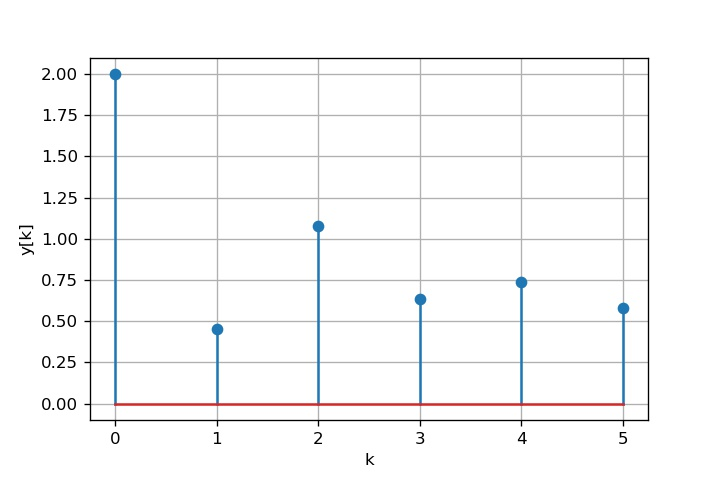
\includegraphics[width=.5\textwidth]{Img/1-b.jpg}
        \caption{$y[k]$ para los estados inciales $X_0$.}
        \label{fig:1-b}
    \end{figure}

    \subsection*{d)}

    En la Figura \ref{fig:1-d} se observa la evolución de los estados.

    \begin{figure}
        \centering
        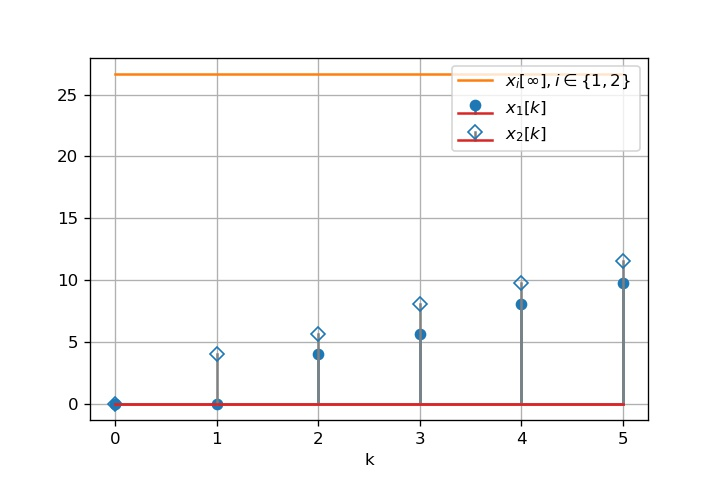
\includegraphics[width=.5\textwidth]{Img/1-d.jpg}
        \caption{Representación de los estados del sistema con respecto a $k$.}
        \label{fig:1-d}
    \end{figure}


    \section*{Ejercicio 2}

    Para este ejercicio se trabajara con 

    \begin{equation}
        H(z) = \frac{1}{z(z-4/5)}
    \end{equation}

    \subsection*{a)}

    Realizando el mismo procedimiento del ejercicio anterior obtenemos que 

    \begin{equation}
        \siseq{
            qX = 
            \begin{bmatrix}
                0 & 1 \\ 
                0 & 4/5
            \end{bmatrix} X
            +
            \begin{pmatrix}
                0 \\ 1
            \end{pmatrix}u \\ 
            Y = 
            \begin{pmatrix}
                1 & 0    
            \end{pmatrix} X
        }
    \end{equation}

    \subsection*{b)}

    Partiendo de que 

    \begin{equation}
        X(0) = 
        \begin{bmatrix}
            0 \\ 0
        \end{bmatrix}
    \end{equation}

    Es posible obtener que 

    \begin{equation}
        X(4) = \Phi^3 \Gamma u[0] + \Phi^2 \Gamma u[1] + \Phi \Gamma u[2] + \Gamma u[3] 
    \end{equation}

    Por lo que la salida en $Y[4]$ esta determinada por 

    \begin{equation}
        Y(4) = x_1[4] = u[2] + \frac{8}{10} u[1] + \frac{16}{25} u[0]
    \end{equation}

    Por lo que una posible secuencia para obtener $Y(4)=5$ es 

    \begin{equation}
        u[k] = 5 \delta[k-2] \lor u[k] = \frac{125}{16} \delta[k]
    \end{equation}

    En la Figura \ref{fig:2-b} puede observarse la salida del sistema partiendo de los estados iniciales nulos. 

    \begin{figure}
        \centering 
        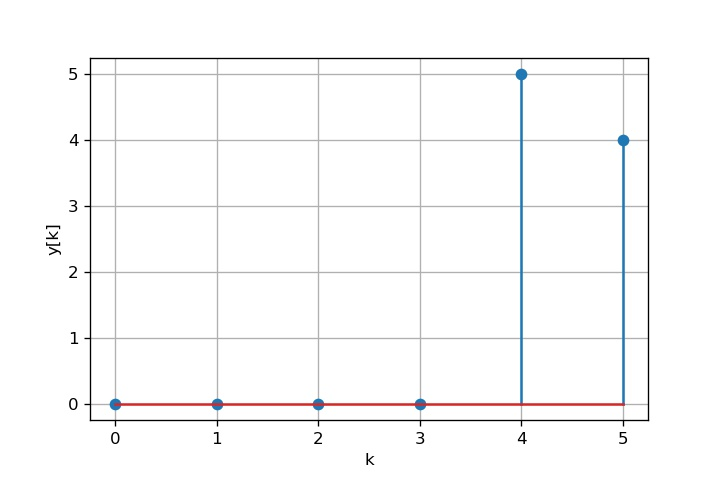
\includegraphics[width=.5\textwidth]{Img/2-b.jpg}
        \caption{$y[k]$ con $X(0)=\vec{0}$ y $u[k]=5\delta[k-2]$.}
        \label{fig:2-b}
    \end{figure}

    \subsection*{c)}

    En la Figura \ref{fig:2-c} se puede observar la evolución de los estados en el plano $(x_1;x_2)$.

    \begin{figure}
        \centering
        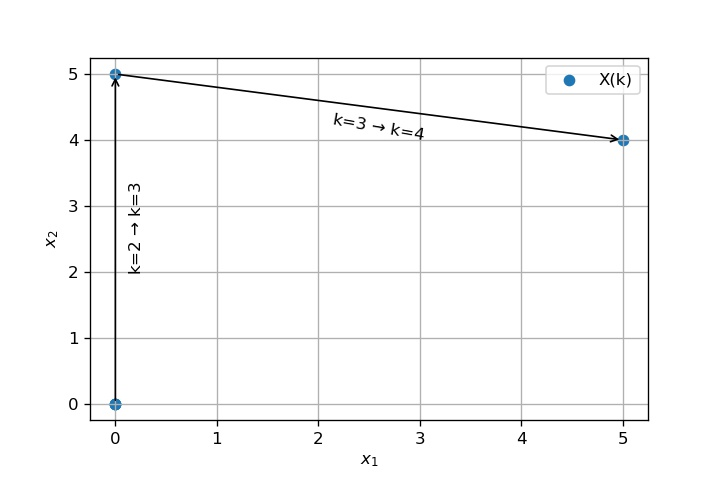
\includegraphics[width=.5\textwidth]{Img/2-c.jpg}
        \caption{Evolución de los estados de $H(z)$.}
        \label{fig:2-c}
    \end{figure}

    \subsection*{d)}

    Para obtener el siguiente vector de estados 

    \begin{equation}
        X[3] = 
        \begin{bmatrix}
            3 \\ 10
        \end{bmatrix}
    \end{equation}

    Partiendo del reposo se obtiene el siguiente sistema 

    \begin{equation}
        X[3] = \Phi^2 \Gamma u[0] + \Phi \Gamma u[1] + \Gamma u[2]
    \end{equation}

    Por lo cual podemos obtener el siguiente sistema de ecuaciones 

    \begin{equation}
        \siseq{
            x_1[3] = 0.8 u_0 + u_1 \\ 
            x_2[3] = 0.64 u_0 + 0.8u_1 + u_2
        } \Leftrightarrow
        \siseq{
            u_1 = - \frac{4}{5}u_0 + 3 \\ 
            u_2 = - \frac{16}{25} u_0 + \frac{16}{25}u_0 - \frac{12}{5} + 10
        }
    \end{equation}

    Por lo tanto una posible solución es 

    \begin{equation}
        u[k] = 3\delta[k-1] + \frac{38}{5} \delta[k-2]
    \end{equation}

    \subsection*{e)}
        La matriz de controlabilidad $W_c$ esta descripta por 
        
        \begin{equation}
            W_c = 
            \begin{bmatrix}
                0 & 1 \\
                1 & 4/5
            \end{bmatrix}
        \end{equation}

        En este caso se observa a simple vista que los vectores columna no son colineales.

        Como los vectores no son colineales entonces en rango de $W_c$ es $2$, por lo tanto el sistema 
        $H(z)$ es controlable.
    \subsection*{f)}

    \section*{Ejercicio 3}

    Para este ejercicio se tiene el siguiente sistema 

    \begin{equation}
        \siseq{
            qX = 
            \begin{bmatrix}
                1/2 & 0 \\ 
                1 & 0
            \end{bmatrix} X
            + 
            \begin{pmatrix}
                0 \\ 1
            \end{pmatrix}u \\ 
            Y = 
            \begin{pmatrix}
                0 & 1
            \end{pmatrix}X
        }
    \end{equation}

    \subsection*{a)}

    Antes de realizar el analisis de los vectores de $W_c$ analizaremos el caso de $\Phi\Gamma$.

    \begin{equation}
        \Phi \Gamma =
        \begin{bmatrix}
            1/2 & 0 \\ 
            1 & 0
        \end{bmatrix}
        \begin{pmatrix}
            0 \\ 1
        \end{pmatrix}
        \Leftrightarrow
        \Phi \Gamma = 
        \begin{pmatrix}
            0 \\ 0
        \end{pmatrix}
    \end{equation}

    Luego como el producto $\Phi^m \Gamma$ puede ser expresado como $\Phi^{m-1}\Phi\Gamma$ entonces 

    \begin{equation}
        \Phi^m\Gamma = \Phi^{m-1} \underbrace{\Phi\Gamma}_{ \vec{0} } = \vec{0}
    \end{equation}

    Por lo tanto todos los vectores columnas de $W_c$ son nulos salvo el primero, por lo tanto son 
    colineares y el rango de $W_c$ es $1$ sin importar el valor de $n$ que se tome.

    Para $n=2$ tenemos que 

    \begin{equation}
        W_c = 
        \begin{bmatrix}
            0 & 0 \\ 
            1 & 0
        \end{bmatrix}
    \end{equation}

    \subsection*{b)}

        Sabemos que los estados finales quedan determinados por 

        \begin{equation}
            X(2) - \Phi^2 X(0) = W_c U \Leftrightarrow
            X(2) = 
            \begin{pmatrix}
                x_1[0] / 4 \\ u[0] + x_2[0] /2
            \end{pmatrix}
        \end{equation}

        En la Figura \ref{fig:3-b} se observa los posible estados finales del sistema.

        \begin{figure}
            \centering 
            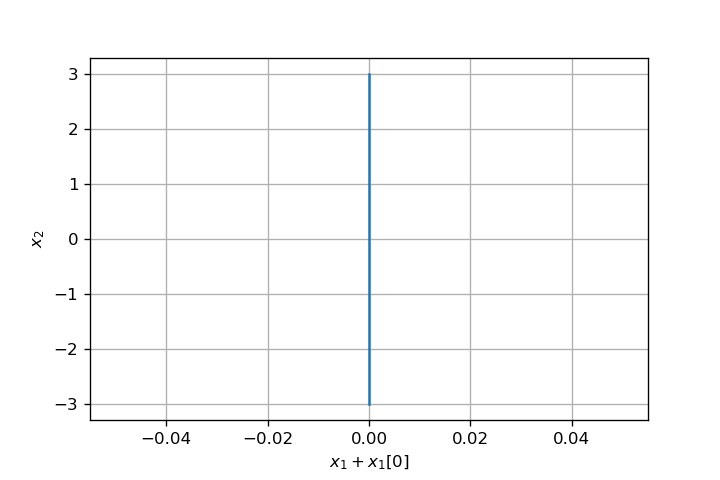
\includegraphics[width=.5\textwidth]{Img/3-b.jpg}
            \caption{Representación de $(x_1;x_2)$ luego de $2$ pasos.}
            \label{fig:3-b}
        \end{figure} 

    \subsection*{c)}

    No es posible ya que por las ecuciones presentadas en el inciso anterior podemos concluir que 
    el sistema no es controlable al origen debido a que el estado $x_1$ tiene siempre el mismo valor,
    el cual es definido por el estado inicial del sistema.

    \subsection*{d)}

    No, como existe una variación de signo en $x_1$ y por lo explicado en el inciso anterior no 
    es posible llegar de un estado $X(0)$ a un $X(M)$ si existe una variación del estado 
    $x_1$.

    \section*{Ejercicio 4}

    Para este ejercicio se cuenta con 

    \begin{equation}
        qX = 
        \begin{bmatrix}
            0 & 1 & 2 \\ 
            0 & 0 & 3 \\ 
            0 & 0 & 0 
        \end{bmatrix} X 
        + 
        \begin{pmatrix}
            0 \\ 1 \\ 0
        \end{pmatrix} u
    \end{equation}

    \subsection*{a)}

    Como primer paso calcularemos $\Phi^n$ entonces 

    \begin{equation}
        \Phi^2 = 
        \begin{bmatrix}
            0 & 0 & 3 \\ 
            0 & 0 & 0 \\
            0 & 0 & 0 
        \end{bmatrix}
    \end{equation}
    
    \begin{equation}
        \Phi^n = 0_{3x3} , n \geq 3
    \end{equation}



    Por lo tanto 

    \begin{equation}
        W_c = 
        \begin{bmatrix}
            0 & 1 & 0 & \cdots & 0 \\ 
            1 & 0 & 0 & \cdots & 0 \\ 
            0 & 0 & 0 & \cdots & 0 
        \end{bmatrix}
    \end{equation}

    Luego podemos calculal el valor de la secuencia $U$ que consigue los estados finales a partir de 
    un estado inicial dado como 

    \begin{equation}
        X(n) - \underbrace{\Phi^n}_{0_{3x3}} X(0) = W_c U
    \end{equation}

    Con lo que obtenemos 

    \begin{equation}
        \label{eq:3-x-n}
        X(n) = 
        \begin{pmatrix}
            u_1 \\ u_0 \\ 0
        \end{pmatrix}
    \end{equation}

    De la ecuación anterior podemos observar que el sisitema es controlable al origen.
    Pero no es controlable de forma completa ya que un estado es siempre nulo.


    \subsection*{b)}

    El $n$ minimo con el que logramos llevar al origen al es $2$ ya que un estado es siempre nulo.

    \subsection*{c)}

    De la ecuación \ref{eq:3-x-n} se puede observar que un estado final siempre debe ser nulo. Por 
    lo tanto si partimos de cualquier estado no es posible llegar a 

    \begin{equation}
        X(M) = 
        \begin{pmatrix}
            1 \\ 1 \\ 1
        \end{pmatrix}
    \end{equation}

    \section*{Ejercicio 5}

    El sistema esta descripto por 

    \begin{equation}
        \siseq{
            qX = 
            \begin{bmatrix}
                1/2 & -1/2 \\
                0 & 5/4
            \end{bmatrix} X
            +
            \begin{pmatrix}
                6 \\ 4
            \end{pmatrix} u \\ 
            Y = 
            \begin{pmatrix}
                2 & -4
            \end{pmatrix} X
        }
    \end{equation}
    
    \subsection*{a)}

    Como el sistema es de orden $2$ entonces 

    \begin{equation}
        W_c = 
        \begin{bmatrix}
            \Gamma & \Phi \Gamma
        \end{bmatrix}
    \end{equation}

    Entonces 

    \begin{equation}
        \Phi \Gamma = 
        \begin{pmatrix}
            1 \\ 5
        \end{pmatrix}
    \end{equation}

    Por lo tanto 

    \begin{equation}
        W_c = 
        \begin{bmatrix}
            6 & 1 \\ 
            4 & 5
        \end{bmatrix}
    \end{equation}

    Como $|W_c| = 26 \neq 0$ entonces existe $W_c^{-1}$, por lo tanto el sistema es controlable.

    \subsection*{b)}

    La matriz de observabilidad esta determinada por 

    \begin{equation}
        W_o = 
        \begin{bmatrix}
            C \\ C\Phi
        \end{bmatrix}
    \end{equation}

    En este caso 

    \begin{equation}
        C \Phi = 
        \begin{pmatrix}
            1 & -6
        \end{pmatrix}
    \end{equation}

    Finalmente se tiene que 

    \begin{equation}
        W_o = 
        \begin{bmatrix}
            2 & -4 \\
            1 & -6
        \end{bmatrix}
    \end{equation}

    Cuyo determinante es $|W_o|=-8$ por lo tanto el sistema es observable.

    \subsection*{c)}

    Para determinar los polos del sistema primero calcularemos el polinomio caracteristo de $\Phi$
   
   \begin{equation}
       P(\lambda) = |\lambda I - \Phi| = 
       \begin{vmatrix}
        \lambda - 1/2 & 1/2 \\
        0 & \lambda - 5/2   
       \end{vmatrix} = 
       (\lambda - 1/2)(\lambda - 5/2)
   \end{equation}

   Podemos observar que sus polos se encuentras en $\{1/2;5/2\}$ como 1 de ellos se encuentra fuera del 
   circulo unitario entonces el sistema es inestable.

    \section*{Ejercicio 6}

   En este ejercicio se tiene el siguiente sistema 

   \begin{equation}
       \siseq{
           qX = 
           \begin{bmatrix}
               1 & 0 \\ 
               0 & 1/2
           \end{bmatrix}X 
           +
           \begin{pmatrix}
               1 & 1 \\ 
               1 & 0
           \end{pmatrix} u \\
           Y = 
           \begin{pmatrix}
               1 & 0
           \end{pmatrix} X
       }
   \end{equation}

   Para saber si el sistema es controlable debemos analizar el rango de $W_o$. 
   Luego como primer paso calcularemos $W_o$

   \begin{equation}
       W_o = 
       \begin{bmatrix}
           \Gamma & \Phi \Gamma
       \end{bmatrix}
   \end{equation}

   Entonces 

   \begin{equation}
       \Phi \Gamma = 
       \begin{bmatrix}
           1 & 1 \\
           1/2 & 0
       \end{bmatrix}
   \end{equation}

   Por lo tanto 

   \begin{equation}
       W_o = 
       \begin{bmatrix}
           1 & 1 & 1 & 1 \\
           1 & 0 & 1/2 & 0
       \end{bmatrix}
   \end{equation}

   Como las filas de $W_o$ no son colineales entonces el rango de $W_o$ es $2$ entonces el sistema es controlable.

   Al realizar el cambio de variable $u = \begin{pmatrix} 1 & 1 \end{pmatrix}^T u_1$ entonces se obtiene el sistema

   \begin{equation}
    \siseq{
        qX = 
        \begin{bmatrix}
            1 & 0 \\ 
            0 & 1/2
        \end{bmatrix}X 
        +
        \begin{pmatrix}
            2 \\ 1
        \end{pmatrix} u_1 \\
        Y = 
        \begin{pmatrix}
            1 & 0
        \end{pmatrix} X
    }
   \end{equation}

   \textbf{PREGUNTAR!!!}

    \section*{Ejercicio 7}

   Del sistema generico de orden 2 

   \begin{equation}
       \siseq{
           qX = 
           \begin{bmatrix}
               a_{11} & a_{12} \\
               a_{21} & a_{22}
           \end{bmatrix} X
           +
           \begin{pmatrix}
               b_1 \\ b_2
           \end{pmatrix} u \\ 
           Y = 
           \begin{pmatrix}
               c_1 & c_2
           \end{pmatrix} X
       }
   \end{equation}

   \subsection*{a)}

   Si utilizamos un controlador del tipo $u=-LX$ entonces 

   \begin{equation}
       \siseq{
           qX = 
           \begin{bmatrix}
               a_{11} - b_1l_1 & a_{12} - b_1l_2 \\
               a_{21} - b_2l_1 & a_{22} - b_2l_2 \\
           \end{bmatrix}X \\
           Y = 
           \begin{bmatrix}
               c_1 & c_2
           \end{bmatrix} X
       }
   \end{equation}

   Sabemos que los polos del sistema estas definidos por los autovalores de la matriz $\Phi$. 
   entonces plantearemos dicho polinomio 

   \begin{equation}
       P(\lambda) = 
       \begin{vmatrix}
           \lambda I - \Phi_{LC}
       \end{vmatrix} = 
       \lambda ^ 2 
       + 
       [b_1l_1 - (a_{11} + a_{22})]\lambda
       + (b_2l_2-a_{22})(b_1l_1 - a_{11}) - (b_2l_1 - a_{21})(b_1l_2 - a_{12})
   \end{equation}

   Como el polinomio que queremos es 

   \begin{equation}
       P(\lambda) = \lambda^2
   \end{equation}

   Entonces es posible obtener el siguiente sistemas de ecuaciones 

   \begin{equation}
    \label{eq:7-zeros}
       \siseq{
           b_1l_1 + b_2l_2 = a_{11} + a_{22} \\ 
           (b_2a_{12} - a_{22}b_1 ) l_1 + 
           (b_1a_{21} - a_{11}b_2) l_2 = - |\Phi|
       }
   \end{equation}

   \subsection*{b)}

   Sabemos que el sistema del ejercicio 1 esta descripto por la ecuación \ref{eq:1-VE}. Remplazando en 
   el la ecuación \ref{eq:7-zeros} los valores de $a_{ij}$ y $b_i$ obtenemos que 

   \begin{equation}
       \siseq{
           4l_2 = \frac{2}{5} \\ 
           4l_1 = \frac{9}{20}
       }
       \Leftrightarrow
       \siseq{
           l_1 = \frac{9}{80} \\ 
           l_2 = \frac{1}{10}
       }
   \end{equation}


   \subsection*{c)}

   En la Figura \ref{fig:7-c} puede observarse la evolución de $y[k]$ para una entrada escalon unitario.
   Donde se observa que se alcanza el estado estacionario en $2$ pasos. 

   \begin{figure}
       \centering
       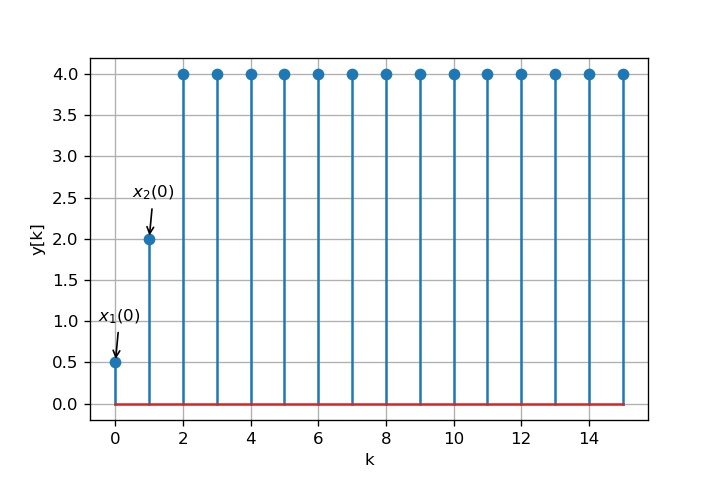
\includegraphics[width=.7\textwidth]{Img/7-c.jpg}
       \caption{Salida del sistema del ejercicio 1 con estados iniciales $X(0)=[1/2 2]^T$ con una entrada escalon unitario.}
       \label{fig:7-c}
   \end{figure}

    \section*{Ejercicio 8}

       Para este ejercicio se tiene el sistema 
       
       \begin{equation}
           \siseq{
               qX = 
               \frac{1}{10}
               \begin{bmatrix}
                   5 & 6 \\
                   3 & 10
               \end{bmatrix} X +
               \begin{pmatrix}
                   1 \\ 0
               \end{pmatrix} u \\ 
               Y = 
               \begin{pmatrix}
                   1 & 0
               \end{pmatrix} X
           }
       \end{equation}


       \subsection*{a)}

       El polinomio caracteristico a lazo cerrado deseado es 

       \begin{equation}
           P_{LC}(\lambda) = \lambda^2 - \frac{7}{20} \lambda + \frac{1}{40}
       \end{equation}

       Sabemos que para una retroalimentación de estados de la forma $u=-LX$ obtenemos que 
       
       \begin{equation}
           \Phi_{LC} = \frac{1}{10} \Phi - BL \Leftrightarrow
           \Phi_{LC} = 
           \begin{bmatrix}
               1/2 - l_1 & 3/5 - l_2 \\
               0.3 & 1
           \end{bmatrix}
       \end{equation}


       El polinomio caracterisco esta dado por 

       \begin{equation}
           P(\lambda) = \lambda^2 + \left( l_1 - \frac{3}{2} \right) \lambda \left( 
               \frac{8}{25} - l_1 + \frac{3}{10}l_2
            \right)
       \end{equation}

       Por lo tanto obtenemos el siguiente sistema de ecuaciones 

       \begin{equation}
           \siseq{
               l_1 - \frac{3}{2} = -\frac{7}{20} \\ 
               \frac{3}{10}l_2 - l_1 + \frac{8}{25} = \frac{1}{40}
           } \Leftrightarrow
           \siseq{
               l_1 = \frac{23}{20} \\ 
               l_2 = \frac{57}{20}
           }
       \end{equation}

    \subsection*{b)}

       Para ubicar ambos polos en el origen, es posible utilizar la ecuación \ref{eq:7-zeros}. Para 
       este caso particular obtenemos 

       \begin{equation}
           \siseq{
               l_1 = \frac{3}{5} \\ 
               -\frac{1}{10}l_1 + \frac{3}{10}l_2 = \frac{13}{100}
           } \Leftrightarrow
           \siseq{
               l_1 = \frac{3}{5} \\ 
               l_2 = \frac{19}{30}
           }
       \end{equation}

    \subsection*{c)}

    En la Figura \ref{fig:8-c} se observan los graficos para los $2$ controladores. En la salida del controlador de a) se 
    observa una oscilación debida al valor de los polos. Por otro lado el estado transitorio es mucho mas largo en el caso 
    del controlador a esto se debe a que los polos del b estan en $0$ lo que produce la mayor velocidad posible.
    En ambas señales se observa que los valores para $k=0$ y $k=1$ son los mismos y varían segun los estados 
    iniciales del sistema.

    \begin{figure}
        \centering
        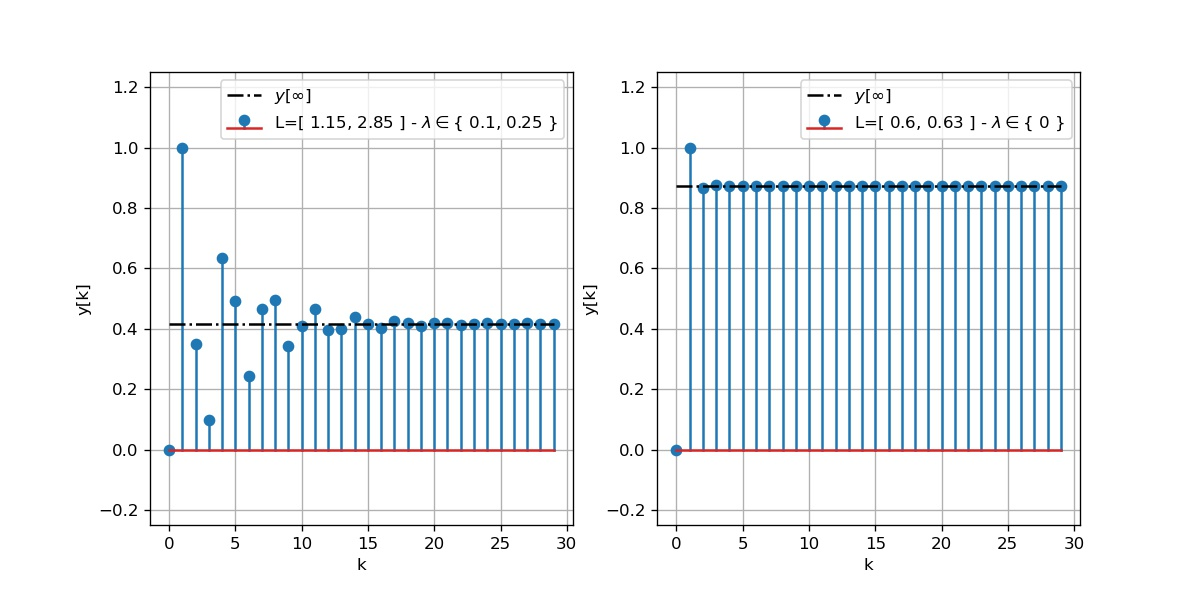
\includegraphics[width=\textwidth]{Img/8-c.jpg}
        \caption{$y[k]$ para los distintos controladores.}
        \label{fig:8-c}
    \end{figure}

    \section*{Ejercicio 9}

    Para este ejercicio se trabajara con 

    \begin{equation}
        \siseq{
            qX = 
            \begin{bmatrix}
                e^{-h} & 0 \\ 
                1-e^{-h} & 1
            \end{bmatrix} X
            + 
            \begin{pmatrix}
                1 - e^{-h} \\ 
                h - 1 + e^{-h}
            \end{pmatrix} u \\ 
            Y = 
            \begin{pmatrix}
                0 & 1
            \end{pmatrix} X
        }
    \end{equation}

    Con estado inicial 

    \begin{equation}
        X(0) = 
        \begin{bmatrix}
            1 \\ 1
        \end{bmatrix}
    \end{equation}

    Cuyo polinomio caracteristico es 
    
    \begin{equation}
        P(\lambda) = (\lambda - e^{-h})(\lambda - 1)
    \end{equation}

    \subsection*{a)}

    Del polinomio caracteristico podemos observar que para cualqueir valor de $h$ el sistema tiene un polo en $1$, lo que conlleva 
    a que el sistema sea inestable.
    
    \subsection*{b)}

    Sabiendo que la señal de control es $u[k]=-Lx[k]$ y sabiendo que el maximo se da en $k=0$, entonces 
    
    \begin{equation}
        |u[0]| \leq 1 \Leftrightarrow |-Lx[0]| \leq 1 \Leftrightarrow
        |l_1 + l_2 |\leq 1 
    \end{equation}

    Si suponemos que $l_i \geq 0, i \in \{1, 2\}$, entonces la condicion a cumplir es 

    \begin{equation}
        l_1 + l_2 \leq 1
    \end{equation}

    \subsection*{c)}


    \section*{Ejercicio 10}


        Para este ejercicio se trabajara con $h=0.25$ por lo que obtenemos 

        \begin{equation}
            \siseq{
                qX = 
                \begin{bmatrix}
                    e^{-1/4} & 0 \\
                    a & 1 
                \end{bmatrix} X 
                + 
                \begin{pmatrix}
                    a \\ h - a
                \end{pmatrix} u \\
                Y = 
                \begin{pmatrix}
                    0 & 1
                \end{pmatrix}X
            }, a = 1 - e^{-1/4}
        \end{equation}

    \subsection*{a)}

        En este caso debemos calcular el estimador de la forma 
        
        \begin{equation}
            \hat{x}[k] = \Phi^{n-1}W_o^{-1} 
            \begin{bmatrix}
                y[k - n + 1] \\ 
                y[k - n + 2] \\ 
                \vdots \\
                y[k]
            \end{bmatrix}
            + \Psi 
            \begin{bmatrix}
                u[k - n + 1] \\ 
                u[k - n + 2] \\ 
                \vdots \\ 
                u[k-1] 
            \end{bmatrix}
        \end{equation}

        Donde $\Psi$ se obtiene como 
        
        \begin{equation}
            \Psi = [ \Phi^{n-2}\Gamma \Phi^{n-3} \Gamma \cdots \Gamma ] - \Phi^{n-1}W_o^{-1}\Omega
        \end{equation}

        Finalmente llamaremos $W_o$ a la matriz de observabilidad y $\Omega$ esta definida por 

        \begin{equation}
            \Omega = 
            \begin{bmatrix}
                0 & 0 & \cdots & 0 \\ 
                C\Gamma & 0 & \cdots & 0 \\ 
                \vdots & 0 & \cdots & 0 \\ 
                C \Phi^{n-2} \Gamma & C \Phi^{n-3} \Gamma & \cdots & C \Gamma 
            \end{bmatrix}
        \end{equation}

        Donde $n$ es el orden del sistema, en este caso $n=2$, por lo tanto obtenemos 
        
        \begin{equation}
            W_o = 
            \begin{bmatrix}
                0 & 1 \\ 
                a & 1 
            \end{bmatrix}
            \Leftrightarrow
            W_o^{-1} = 
            \begin{bmatrix}
                0 & a^{-1} \\
                1 & -a^{-1}
            \end{bmatrix}
        \end{equation}

        El calculo de $\Omega$ en este caso es sumamente sencillo ya que $n=2$, por lo tanto 

        \begin{equation}
            \Omega = 
            \begin{pmatrix}
                0 \\
                C\Gamma
            \end{pmatrix}
            =
            \begin{pmatrix}
                0 \\
                h-a                
            \end{pmatrix}
        \end{equation}

        Por otro lado el calculo de $\Psi$

        \begin{equation}
            \Psi = 
            \begin{pmatrix}
                a \\ h -a
            \end{pmatrix}
            -
            \begin{bmatrix}
                e^{-1/4} & 0 \\
                a & 1
            \end{bmatrix}
            \begin{bmatrix}
                0 & a^{-1} \\
                1 & -a^{-1}
            \end{bmatrix}
            \begin{pmatrix}
                0 \\
                h-a                
            \end{pmatrix}
            \Leftrightarrow
            \Psi = 
            \begin{pmatrix}
                a - ha^{-1}e^{-1/4} + e^{-1/4} 
                \\ a^{-1}h -1
            \end{pmatrix}
        \end{equation}

        Finalmente el observador posee la forma de 

        \begin{equation}
            \hat{x}[k] = 
            \begin{bmatrix}
                0 & a^{-1}e^{-1/4} \\
                1 & 1 - a^{-1}    
            \end{bmatrix}
            \begin{pmatrix}
                y[k-1] \\ y[k]
            \end{pmatrix}
            +
            \begin{pmatrix}
                a - ha^{-1}e^{-1/4} + e^{-1/4}  \\ a^{-1}h - 1
            \end{pmatrix}
            u[k-1]
        \end{equation}
    
    \subsection*{b)}

    Para el observador dinamico se tiene que 
    
    \begin{equation}
        \Phi_o = \Phi - KC = 
        \begin{bmatrix}
            e^{-1/4} & -K_1 \\
            a & 1 - K_2
        \end{bmatrix}
    \end{equation}

    En este caso se nos pide que el observador tenga los polos en $0$, por lo tanto 
    los autovalores de $\Phi_o$ deben ser nulos, entonces
    
    \begin{equation}
        P(\lambda) = 
        \begin{vmatrix}
            \lambda - e^{-1/4} & -K_1 \\
            a & \lambda - 1 + K_2
        \end{vmatrix} = 
        \lambda ^ 2 + ( K_2 - 1 - e^{-1/4}) \lambda +e^{-1/4} - e^{-1/4}K_2 + K_1a
    \end{equation}

    Por lo tanto 
    
    \begin{equation}
        \siseq{
        K_2 - 1 - e^{-1/4} = 0 \\ 
        e^{-1/4} - e^{-1/4}K_2 + K_1a = 0
        }
        \Leftrightarrow
        \siseq{
            K_1 = - \frac{e^{-1/2}}{1 - e^{-1/4}} \\
            K_2 = 1 + e^{-1/4}
        }
    \end{equation}

    \subsection*{c)}

    En este caso la estimación puede obtenerse como 

    \begin{equation}
        \hat{x}[k|k] = 
        [I - KC][ \Phi \hat{x}[k-1|k-1] + \Gamma u[k-1] ] + Ky[k]
    \end{equation}

    También sabemos que los polos del observador estan determinados por 

    \begin{equation}
        P(\lambda) = | \lambda I - \Phi - KC\Phi |
    \end{equation}

    Entonces $P(\lambda)$ esta expresado por 
    
    \begin{equation}
        P(\lambda) = \lambda^2 - ( e^{-1/4} - K_1a + 1- K_2 )\lambda + (1-K_2)(e^{-1/4} - K_1a ) + K_1( a - K_2 a )
    \end{equation}

    Si ubicamos los polos en $0$ entonces surge el siguiente sistema de ecuaciones

    \begin{equation}
        \siseq{
            e^{-1/4} - K_1a + 1- K_2 = 0 \\ 
            (1-K_2)(e^{-1/4} - K_1a ) + K_1( a - K_2 a ) \\ 
        } \Leftrightarrow
        \siseq{
            K_1 = \frac{e^{-1/4} + 1 - K_2 }{a} \\ 
            e^{-1/4} - K_2 e^{-1/4} = 0
        }
    \end{equation}

    Despejando obtenemos 

    \begin{equation}
        \siseq{
            K_1 = \frac{1}{e^{1/4}-1} \\ 
            K_2 = 1
        }
    \end{equation}


    \section*{Ejercicio 11}

    El sistema del ejercicio 1 es 

    \begin{equation}
        \siseq{
            qX = 
            \begin{bmatrix}
                0 & 1 \\ 
                9/20 & 2/5 
            \end{bmatrix} X +
            \begin{pmatrix}
                0 \\ 4
            \end{pmatrix} u\\ 
            Y = 
            \begin{pmatrix}
                1 & 0     
            \end{pmatrix} X
        }
    \end{equation}

    \subsection*{a)}

    La matriz $\Phi_{LC}$ esta descripto por 
    
    \begin{equation}
        \Phi_{LC} = \Phi - \Gamma L = 
        \begin{bmatrix}
            0 & 1 \\
            \frac{9}{20} - 4l_1 & \frac{2}{5} - 4l_2
        \end{bmatrix}
    \end{equation}

    Cuyo polinomio caracteristo es 

    \begin{equation}
        P(\lambda) = \lambda ^ 2 + \left( 4l_2 - \frac{2}{5} \right) \lambda + 4l_2 - \frac{9}{20}
    \end{equation}

    Como los polos deben estar en $0.5$ entonces se obtiene el siguiente sistema de ecuaciones 

    \begin{equation}
        \siseq{
            4l_2 - \frac{2}{5} = 1 \\
            4l_1 - \frac{9}{20} = \frac{1}{4}
        }
        \Leftrightarrow
        \siseq{
            l_1 = \frac{l_2}{2} \\ 
            l_2 = \frac{7}{20}
        }
    \end{equation}

    \subsection*{b)}

    En este caso $\Phi_o$ esta definida

    \begin{equation}
        \Phi_o = 
        \begin{bmatrix}
            0 & 1 \\
            -\frac{1}{4} & \frac{9}{5}
        \end{bmatrix}
        -
        \begin{pmatrix}
            K_1 \\ K_2
        \end{pmatrix}
        \begin{pmatrix}
            1 & 0
        \end{pmatrix} = 
        \begin{bmatrix}
            -K_1 & 1 \\
            -\frac{1}{4} - K_2 & \frac{9}{5}
        \end{bmatrix}
    \end{equation}

    Cuyo polinomio caracteristico esta dado por 

    \begin{equation}
        P(\lambda) = \lambda^2 + \left( K_1 - \frac{9}{5} \right) \lambda - \frac{9}{5}K_1 + K_2 + \frac{1}{4}
    \end{equation}

    Si los polos del observador deben estar en el origen entonces 

    \begin{equation}
        \siseq{
            K_1 = \frac{9}{5} \\ 
            K_2 = 2.99
        }
    \end{equation}

    \subsection*{c) y d)}

    En la Figura \ref{fig:11} observamos los valores para la salida, en el caso de que sea posible medir $X$ y en el caso 
    de que se necesite estimar $X$ utilizando el observador calculado en b). Por otro lado se observan las variaciones de 
    $x_1$ y $x_2$ en los distintos instantes de tiempo.

    \begin{figure}
        \centering
        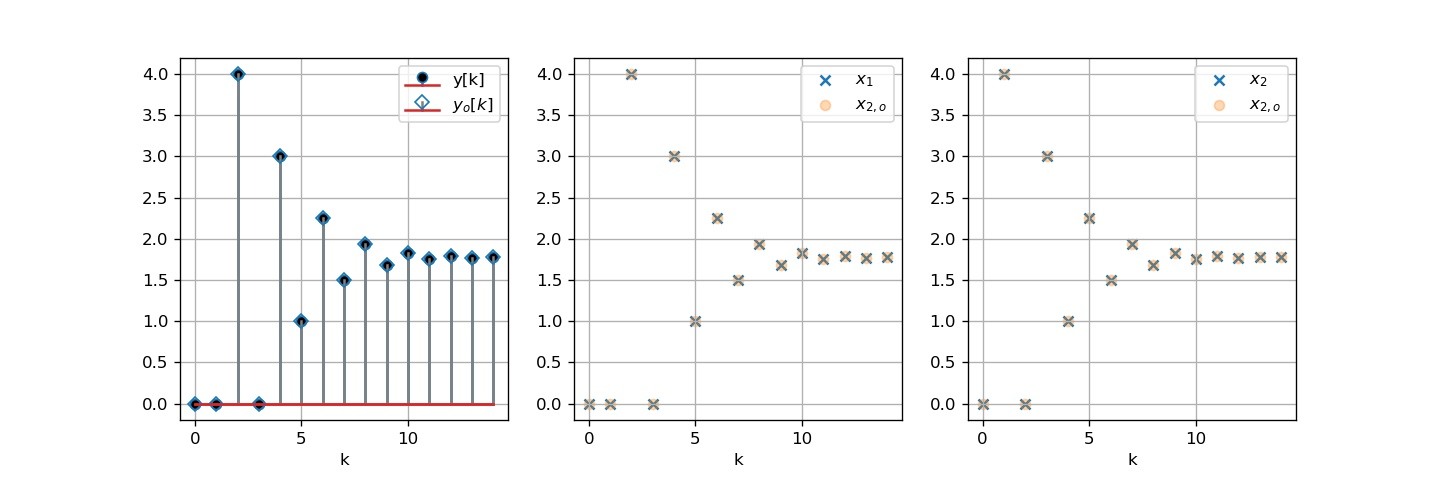
\includegraphics[width=\textwidth]{Img/11-c-d.jpg}
        \caption{Representación de la salida con retroalimentación para los casos en que se pueda medir $X$ y con la implementación del observador dinamico.}
        \label{fig:11}
    \end{figure}

\end{document}